\begin{figure}[t]
    \centering
    % 适当调整宽度以适应页面
    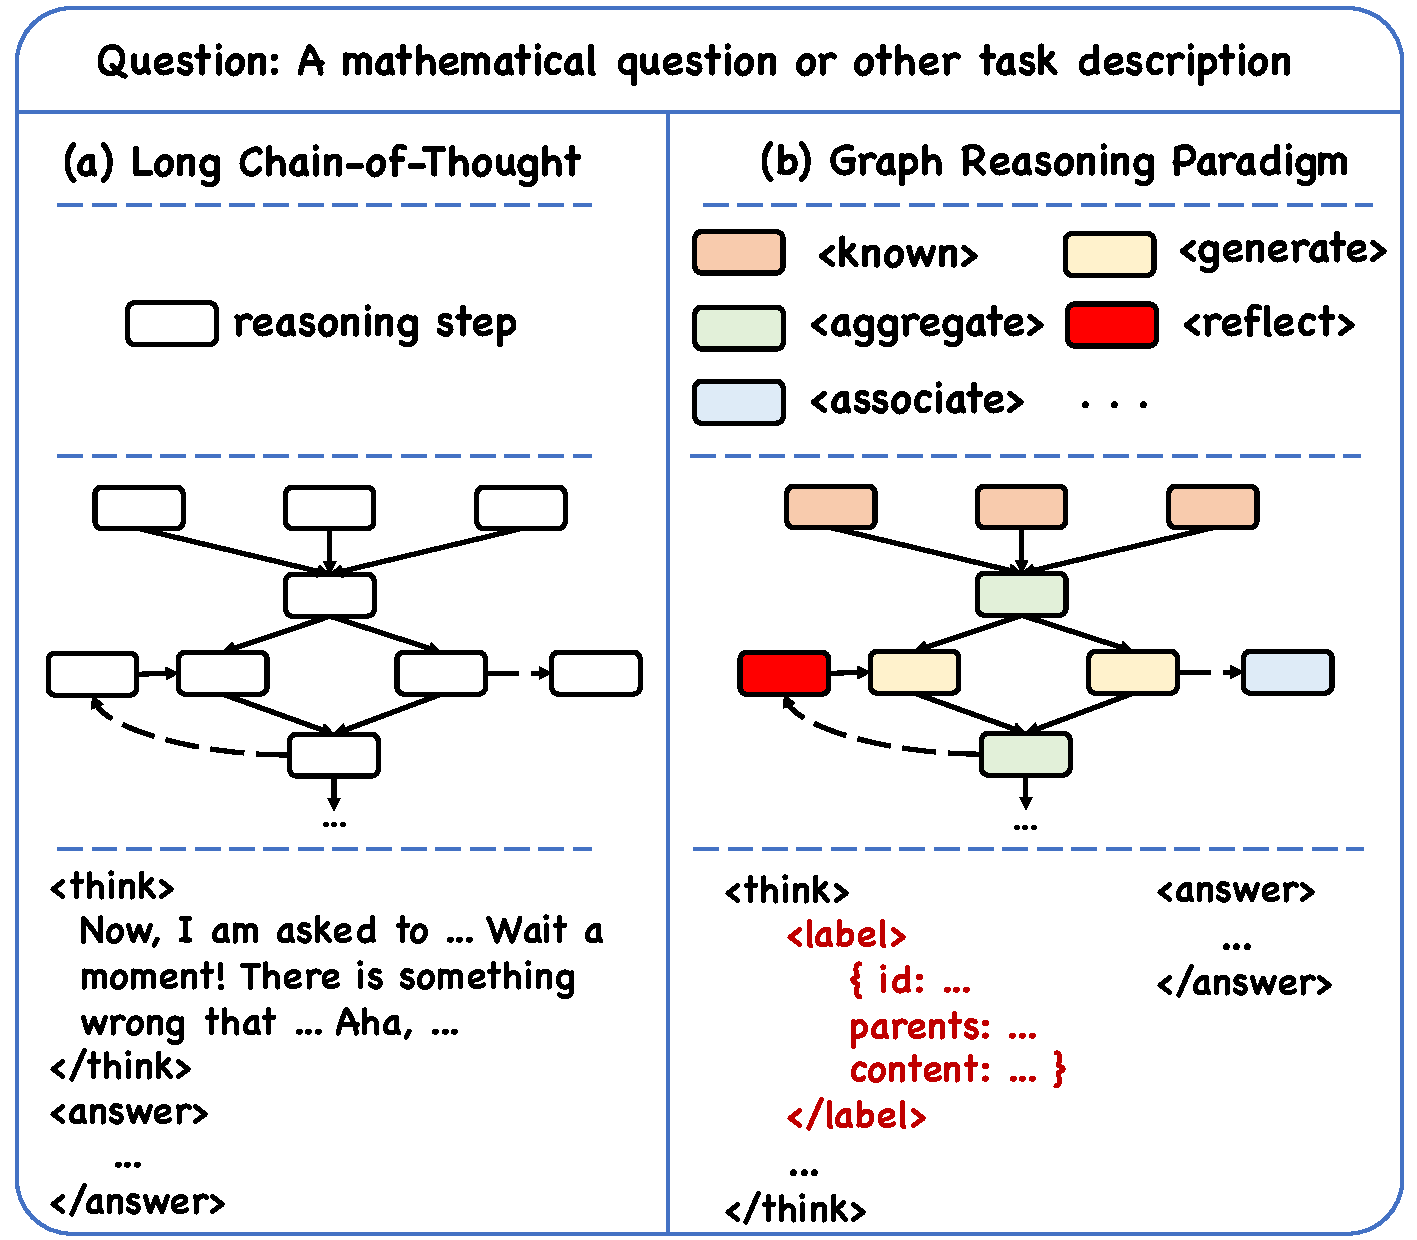
\includegraphics[width=1 \linewidth]{Figures/example-v2_5.pdf}
    \caption{Comparison between traditional Long Chain-of-Thought and Graph Reasoning Paradigm.}
    \label{fig:example}
\end{figure}

Long chain-of-thought (LCoT) has been proven effective for eliciting the reasoning capabilities of Large Language Models (LLMs), particularly when combined with reinforcement learning with verifiable rewards (RLVR)~\cite{ElKishky2024OpenAIOS,Chen2025TowardsRE,He2025BreakingTR}. 
Such approaches have been applied to mathematical reasoning~\cite{Zhou2024SelfDiscoverLL,Moshkov2025AIMO2WS} and code generation~\cite{ElKishky2025CompetitivePW,Yu2025Z1ET}, which are representative complex reasoning tasks and have become common benchmarks for evaluating the reasoning abilities of LLMs.

% 然而，现在大模型输出是纯文本，虽然涌现出了反思和Aha moment这类复杂的思维方式，但是推理过程的可靠性不高。近期有一些强化学习的方法尝试解决这一问题。但是，基于结果奖励的方法，缺少对推理过程语义上的监督。基于过程奖励的方法，虽然把控了推理过程，但是训练成本高，泛化性差。总之，导致这些问题的原因主要来自于语义评估的难度高，现有大模型输出又都是纯文本的，不得不去评估语义，形成死循环。Inspired by the structured cognitive mechanisms of human cognition \cite{George2021ClonestructuredGR}, we argue that 推理过程应该结构化，用结构评估来代替语义评估，实现计算结果奖励时，低成本地评估推理过程。但是过程奖励变多，导致过份追求过程的质量而得不到正确答案，出现了reward hacking现象，这是传统的优势估计方法出现了问题。

However, current LLMs predominantly produce plain-text outputs. Although complex reasoning behaviors such as reflection and Aha moments have emerged \cite{Yang2025UnderstandingAM}, the reliability of the reasoning process remains limited \cite{Shojaee2025TheIO}.
Recently, several reinforcement learning (RL) approaches have attempted to address this issue. However, outcome-based reward methods provide only coarse-grained supervision, offering little semantic control over the reasoning process \cite{DeepSeekAI2025DeepSeekR1IR}. Although process-based reward methods offer semantic control over the reasoning process, they often suffer from high training costs and poor generalization \cite{Yuan2024FreePR}.
In summary, semantic evaluation is inherently difficult. Since LLMs output plain text, we are forced to perform semantic assessments, which creates a vicious cycle.

Inspired by the structured cognitive mechanisms of human cognition \cite{George2021ClonestructuredGR}, we propose to replace plain-text with structured and symbolic representations, and to replace semantic evaluation with structure-based evaluation, thereby enabling low-cost and fine-grained control over the reasoning process when computing outcome rewards.
Notably, increasing reliance on process-based rewards may encourage models to over-optimize intermediate reasoning quality at the expense of correct final answers, giving rise to reward hacking \cite{Denison2024SycophancyTS}. This issue fundamentally reflects the limitations of conventional advantage estimation methods.

In this paper, we propose a \textbf{G}raph \textbf{R}easoning \textbf{P}aradigm (\textbf{GRP}), which realizes the structured and symbolic reasoning process using graph-structured representations.
As shown in Figure~\ref{fig:example}, the reasoning process in this paradigm is explicitly organized into a structured form, where each reasoning step is annotated with a specific cognitive label.
These labels correspond to different cognitive operations, including \emph{known}, \emph{generate}, \emph{aggregate}, \emph{reflect}, \emph{refine}, \emph{reverse}, and \emph{associate}. 
This structured representation transforms reasoning from unstructured text into an explicit graph, improving interpretability, and enabling systematic evaluation of reasoning processes. 
Based on this paradigm, we construct over 40.3k graph-structured mathematical reasoning chains and 12k graph-structured code generation chains with step-level labels, and perform supervised fine-tuning (SFT) to train LLMs to internalize graph-structured reasoning.

Building on the structured and symbolic outputs, we propose \textbf{PASC-GRPO}, a \textbf{P}rocess-\textbf{A}ware \textbf{S}tratified \textbf{C}lipping extension of \textbf{G}roup \textbf{R}elative \textbf{P}olicy \textbf{O}ptimization to further exert finer control over the reasoning process. 
We design a set of graph-based outcome rewards that evaluate the quality of the reasoning process using structural properties such as label validity, reachability, connectivity, informative subgraph, and reverse search consistency. 
These rewards do not rely on value models for semantic evaluation, leading to better generalization and improved training efficiency. 
To mitigate reward hacking introduced by multiple rewards, we further propose stratified clipping advantage estimation, which separately normalizes rewards within correct and incorrect groups, ensuring stable and reliable optimization.

% Experiments are conducted on mathematical reasoning and code generation benchmarks. The results show consistent improvements in accuracy and efficiency.

Experiments across mathematical reasoning and code generation benchmarks demonstrate that our method consistently outperforms strong baselines, particularly on competition-level tasks. Furthermore, it effectively mitigates reward hacking and reduces reasoning length, improving both accuracy and inference efficiency. In summary, our contributions are threefold:
\begin{itemize}
    \item We propose a \textbf{Graph Reasoning Paradigm} that enables structured and symbolic reasoning processes. We construct over \textbf{52k} graph-structured reasoning chains with step-level cognitive labels for SFT.
    \item We propose \textbf{PASC-GRPO}, a reinforcement learning method that leverages graph-structured outcome rewards and stratified clipping advantage estimation to improve reasoning quality while mitigating reward hacking.
    \item We empirically demonstrate that our approach significantly improves the reasoning performance of LLMs, providing evidence for the effectiveness of graph reasoning paradigm.
\end{itemize}

% Long Chain-of-Thought (LCoT) reasoning has been shown to effectively elicit the reasoning capabilities of LLMs \cite{ElKishky2024OpenAIOS,Chen2025TowardsRE,He2025BreakingTR}. LCoT has been widely applied to mathematical reasoning \cite{Zhou2024SelfDiscoverLL,Moshkov2025AIMO2WS} and code generation \cite{ElKishky2025CompetitivePW,Yu2025Z1ET}, which are representative complex reasoning tasks and have become common benchmarks for evaluating the reasoning abilities of LLMs.

% However, the existing thinking process in LLMs is predominantly text-based, lacking explicit representations of reasoning paths and logical structure. 
% Such linear textual reasoning obscures the dependencies among the reasoning steps, making complex reasoning difficult to trace, verify, and control. 
% In addition, outcome-based reward methods \cite{Shao2024DeepSeekMathPT,DeepSeekAI2025DeepSeekR1IR} lack fine-grained supervision over the reasoning process and are vulnerable to reward hacking \cite{Denison2024SycophancyTS}. 
% Process-based reward methods \cite{Lightman2023LetsVS,Zhang2025DreamPRMCodeFP} provide more fine-grained supervision, but typically suffer from limited generalization and incur substantial training overhead.
% % 受人类结构化学习和思考机制启发，我们认为模型的训练和推理过程应该显式地建模为图
% Inspired by the structured cognitive mechanisms of human cognition \cite{George2021ClonestructuredGR}, we argue that the training and inference processes should be explicitly modeled as graph structures, enabling the traceability and optimization of thinking paths.


% \begin{figure}[t]
%     \centering
%     % 适当调整宽度以适应页面
%     
\includegraphics[width=1 \linewidth]{example.pdf}
%     \caption{Heatmap illustrating the prevalence of graph-structured reasoning in success cases of strong models (where weak models failed). The intensity of the color and the annotated values indicate the proportion of responses containing graph patterns across different tasks and difficulty levels. The visual gradient highlights the increased necessity of graph reasoning for harder problems.}
%     \label{fig:empirical_analysis}
% \end{figure}

% \begin{figure}[t]
%     \centering
%     % 适当调整宽度以适应页面
%     \includegraphics[width=1 \linewidth]{Figures/example-v2_3.pdf}
%     \caption{Comparison between traditional Long Chain-of-Thought and Graph Reasoning Paradigm.}
%     \label{fig:example}
% \end{figure}

% Through empirical analysis, we observe that Long Chain-of-Thought (LCoT) often exhibits graph-structured reasoning patterns, such as divide-and-conquer, aggregation, and reflection. As illustrated in Figure~\ref{fig:example}, stronger models tend to employ these graph-structured patterns more frequently in cases where they succeed but weaker models fail. This observation suggests that graph-structured reasoning may play an important role in effective problem solving, motivating a more explicit modeling of such structures.

% Several prior works have attempted to leverage graph-structured reasoning. For example, Graph-of-Thought \cite{Besta2023GraphOT} organizes reasoning steps into graph-like structures by prompt engineering, treating LLMs as executors and evaluators. Although effective in some settings, these approaches rely heavily on manually designed prompts and external control logic. As a result, the graph structure is not learned as an intrinsic reasoning capability of the model, and generalization across tasks and domains remains limited.

% However, existing reasoning in LLMs is predominantly text-based, lacking explicit representations of reasoning paths and logical structure. Such linear textual reasoning obscures the dependencies among the reasoning steps, making complex reasoning difficult to trace, verify, and control. In contrast, human reasoning is inherently structured and often exhibits non-linear patterns with branching, aggregation, and feedback \cite{Forstmann2016SequentialSM,Ball2022TheRI}. Motivated by this gap, we argue that reasoning should be explicitly modeled as a graph, where nodes represent reasoning steps, and edges encode their logical dependencies, enabling more interpretable, verifiable, and logically consistent reasoning in LLMs.

% In parallel, reinforcement learning (RL) has recently shown promising results in improving the reasoning performance of LLMs. Despite recent progress, outcome-based reward methods \cite{Shao2024DeepSeekMathPT,DeepSeekAI2025DeepSeekR1IR} lack fine-grained supervision over the reasoning process and are prone to reward hacking \cite{Denison2024SycophancyTS}. Process-based reward methods \cite{Lightman2023LetsVS,Zhang2025DreamPRMCodeFP} provide more fine-grained supervision, but typically suffer from limited generalization and incur substantial training overhead.

% To address these challenges, in this work, we propose a \textbf{G}raph \textbf{R}easoning \textbf{P}aradigm (\textbf{GRP}) to explicitly model complex human cognition in LLM reasoning. 